\documentclass[class=minimal,border=0pt]{standalone}
\usepackage{tikz}
\usepackage{amsmath}

\usetikzlibrary{%
  arrows,
  calc
}
\usetikzlibrary{decorations.markings}
\usetikzlibrary{shapes.misc}

\begin{document}
  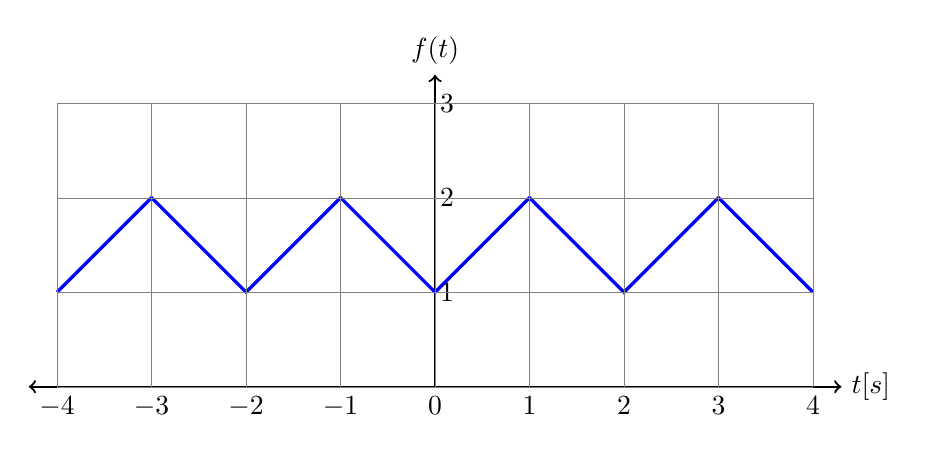
\begin{tikzpicture}[yscale=1.2, xscale=1.2]
    \draw[<->,thick] (-4.3,0) -- (4.3,0) node[right] {$t[s]$};
    \draw[->,thick] (0,0) -- (0,3.3) node[above] {$f(t)$};

    \draw[line width = 1.2pt, blue] (-4,1) -- (-3,2) -- (-2,1)
    --  (-1,2) -- (0,1) -- (1,2)--(2,1)--(3,2)--(4,1);    
    
 
    \draw (-1,0) node[below] {$-1$};
    \draw (1,0) node[below] {$1$};
    \draw (-2,0) node[below] {$-2$};
    \draw (2,0) node[below] {$2$};
    \draw (3,0) node[below] {$3$};
    \draw (-3,0) node[below] {$-3$};
    \draw (4,0) node[below] {$4$};
    \draw (-4,0) node[below] {$-4$};
    \draw (0,0) node[below] {$0$};
    
	\draw (-0.05,3) node[right] {$3$};
    \draw (-0.05,2) node[right] {$2$};
    \draw (-0.05,1) node[right] {$1$};
    
    
    

    \draw[step=1cm,color=gray, ultra thin] (-4,0) grid (4,3);

  \end{tikzpicture}

\end{document}